\documentclass[11pt,a4paper]{article}
\usepackage[T1]{fontenc}
\usepackage[utf8]{inputenc}
\usepackage{lmodern}
\usepackage{amsmath,amsthm,amssymb,mathtools}
\usepackage[margin=25mm,headheight=15pt]{geometry}
\usepackage{microtype,booktabs,array,enumitem,xcolor}
\usepackage{tikz}
\usetikzlibrary{positioning}
\usepackage{listings}
\usepackage[colorlinks=true,linkcolor=blue!45!black,citecolor=blue!45!black,urlcolor=blue!50!black]{hyperref}
\usepackage{fancyhdr}
\setlength{\emergencystretch}{3em}
\pagestyle{fancy}\fancyhf{}\lhead{Parity-to-certificate transfer}\rhead{Research draft -- 16 November 2026}\cfoot{\thepage}
\newtheorem{theorem}{Theorem}[section]
\newtheorem{lemma}[theorem]{Lemma}
\newtheorem{proposition}[theorem]{Proposition}
\newtheorem{corollary}[theorem]{Corollary}
\newtheorem{problem}[theorem]{Auxiliary problem}
\theoremstyle{definition}\newtheorem{definition}[theorem]{Definition}
\newtheorem{example}[theorem]{Example}
\theoremstyle{remark}\newtheorem{remark}[theorem]{Remark}
\newcommand{\Gbar}{\overline G}
\newcommand{\TDS}{\mathrm{TDS}}
\newcommand{\epar}{\mathsf E}
\newcommand{\trans}{\mathsf T}
\newcommand{\compdef}{\mathsf c}
\newcommand{\N}{\mathbb N}
\newcommand{\V}{V(G)}
\newcommand{\WTD}{\mathrm{WTD}}
\definecolor{navy}{HTML}{133457}
\definecolor{slate}{HTML}{556779}
\lstset{basicstyle=\ttfamily\scriptsize,breaklines=true,breakatwhitespace=false,frame=single,rulecolor=\color{gray!50},columns=fullflexible,showstringspaces=false,keepspaces=true,aboveskip=12pt,belowskip=12pt}
\hypersetup{pdftitle={Parity-to-Certificate Transfer: Global Proofs of Written on the Wall II Conjectures 318 and 320},pdfauthor={Research notes for Keio},pdfsubject={Graph theory, total domination, graph complements, conjecture audit}}
\title{\textcolor{navy}{Parity-to-Certificate Transfer}\\[5pt]
\large Two Global Proofs for \emph{Written on the Wall II} Conjectures 318 and 320, with a Sharp Complement-Concentration Theorem}
\author{Research manuscript prepared for Keio\\[4pt]\small Independent verification and priority review requested}
\date{16 November 2026}
\begin{document}
\maketitle
\begin{abstract}
In the \emph{Written on the Wall II} collection, Graffiti.pc Conjecture 318 (4 March 2007) states that a connected simple graph is well-totally-dominated when its maximum even-distance vertex count is at least the number of missing edges. Conjecture 320 (the same date) asserts the same conclusion when the maximum even-distance vertex count equals the minimum vertex transmission. Both are marked open in the maintainer's 5 November 2026 update. We give self-contained, unconditional proofs of the original implications. The principal auxiliary problem is resolved with a sharp global theorem: if a connected graph has $m$ missing edges and its complement has maximum degree $d$, then $m-d\le 1$ forces \emph{every} inclusion-minimal total dominating set to have exactly two vertices; the threshold cannot be relaxed to $2$. The proof uses a two-vertex domination certificate extracted from an arbitrary total dominating set. For Conjecture 320 we establish the exact equality classification: the equality between the two metric invariants occurs precisely when the graph has both a universal vertex and a pendant vertex. Neither argument uses a finite-order hypothesis, a numerical approximation, or an unproved auxiliary conjecture. An independent Graph Atlas census checks all 995 connected nonisomorphic graphs with 2--7 vertices. \emph{Novelty is not certified}: an indexed literature search did not identify an identical earlier resolution, but this is not evidence of absolute publication priority; the work remains a preprint pending expert examination.
\end{abstract}
\noindent\textbf{Keywords:} total domination, well-totally-dominated graphs, even-distance layers, graph complement, structural certificates, Graffiti.pc.\\
\textbf{MSC 2020:} 05C69, 05C75, 05C12.
\tableofcontents

\section{Original problems and scope}
The source of the questions is Ermelinda DeLaVi\~na's \emph{Written on the Wall II -- Conjectures of Graffiti.pc}, a dated list of machine-generated graph conjectures \cite{DeLaVina2026}. The publicly listed status, as updated on 5 November 2026 and printed on 6 November 2026, is \emph{open} for entries 318 and 320. We do not infer publication priority from that status.

Throughout, $G$ is a finite, simple, connected, undirected graph with $n:=|\V|\ge2$. Distances are ordinary shortest-path distances. The complement $\Gbar$ has the same vertex set and exactly the nonedges of $G$. Write
\begin{align}
 m(G)&:=|E(\Gbar)|, & d(G)&:=\Delta(\Gbar), & \compdef(G)&:=m(G)-d(G),\label{eq:defect}\\
 \epar_G(v)&:=|\{u\in\V:d_G(u,v)\text{ is even}\}|, &
 \epar(G)&:=\max_{v\in\V}\epar_G(v),\label{eq:even}\\
 \trans_G(v)&:=\sum_{u\in\V}d_G(u,v), &
 \trans(G)&:=\min_{v\in\V}\trans_G(v).\label{eq:transmission}
\end{align}
As in the source definitions, $d_G(v,v)=0$ counts as an even distance, so $v$ itself contributes one to $\epar_G(v)$. Since $G$ is connected, all sums are finite.

A set $D\subseteq\V$ is a \emph{total dominating set} if every vertex, \emph{including each member of $D$}, has a neighbor in $D$. It is \emph{minimal} if no proper subset is a total dominating set, and \emph{minimum} if it has minimum possible cardinality. Denote the minimum size by $\gamma_t(G)$ and the maximum size of an inclusion-minimal total dominating set by $\Gamma_t(G)$. The graph is \emph{well-totally-dominated} if $\gamma_t(G)=\Gamma_t(G)$. This agrees with the original source definition.

\begin{problem}[The unchanged named Conjecture 318, 2007]\label{prob:318}
Prove that for every connected simple graph $G$ of order at least two,
\begin{equation}\label{eq:318}
\epar(G)\ge m(G)\quad\Longrightarrow\quad G\text{ is well-totally-dominated}.
\end{equation}
\end{problem}
\begin{problem}[The unchanged named Conjecture 320, 2007]\label{prob:320}
Prove that for every connected simple graph $G$ of order at least two,
\begin{equation}\label{eq:320}
\epar(G)=\trans(G)\quad\Longrightarrow\quad G\text{ is well-totally-dominated}.
\end{equation}
\end{problem}
These are not newly invented targets: the displayed implications are exactly those recorded in entries 318 and 320, with the original parameters restored rather than replaced. The new quantity $\compdef(G)$ is an auxiliary invariant used to prove, not redefine, the first problem.

\section{The new auxiliary problem: concentrated missing edges}
The methodological starting point is an auxiliary question that asks for a \emph{global} certificate, rather than another metric inequality.

\begin{problem}[Concentrated-complement certificate problem]\label{prob:aux}
Find the largest integer $c$ for which every connected simple $G$ satisfying $m(G)-\Delta(\Gbar)\le c$ has all inclusion-minimal total dominating sets of size two. Give a uniform certificate in an arbitrary total dominating set, and an extremal obstruction showing optimality.
\end{problem}

The difference $m(G)-d(G)$ counts the missing edges \emph{not} incident with a vertex of maximum degree in $\Gbar$. Thus the condition $\compdef(G)\le1$ is not a bound on $m(G)$ itself: there may be arbitrarily many missing edges, as long as all but at most one share a vertex. This distinction is indispensable for the range extension in Section~\ref{sec:range}.

\begin{lemma}[A pair certificate in an almost-complete core]\label{lem:certificate}
Suppose $G$ is connected with $n\ge2$, and some vertex $c$ has the property that the induced graph $G[\V\setminus\{c\}]$ is complete with at most one edge removed. Then every total dominating set $D$ contains a two-element total dominating set. In particular, every minimal total dominating set has size exactly two.
\end{lemma}
\begin{proof}
Put $U=\V\setminus\{c\}$ and $A=N_G(c)$. Connectedness gives $A\ne\varnothing$. Let $D$ be an arbitrary total dominating set. The vertex $c$ is dominated by some $a\in D\cap A$.

\emph{Case 1.} There exists $b\in D\cap(U\setminus\{a\})$ adjacent to $a$. Then $\{a,b\}$ is itself a total dominating set. Indeed $a$ and $b$ dominate each other, $c$ is adjacent to $a$, and any $z\in U\setminus\{a,b\}$ must be adjacent to at least one of $a,b$: otherwise $az$ and $bz$ would be two distinct missing edges of the induced core $G[U]$, contrary to the hypothesis.

\emph{Case 2.} No vertex of $D\cap(U\setminus\{a\})$ is adjacent to $a$. Since $G[U]$ has at most one missing edge, $D\cap U$ is either $\{a\}$ or $\{a,p\}$ for a single possible vertex $p$ with $ap\notin E(G)$. To dominate $a$, the set $D$ must therefore contain $c$. If $p\notin D$, then $D=\{a,c\}$ and is already a two-element total dominating set.

Otherwise $p\in D$. Since $p$ is adjacent neither to $a$ nor to itself, total domination of $p$ by $D=\{a,p,c\}$ forces $pc\in E(G)$. Now $\{a,c\}$ totally dominates: these two vertices are adjacent, $p$ is adjacent to $c$, and every vertex of $U\setminus\{a,p\}$ is adjacent to $a$, because $ap$ is the only possible missing edge within $G[U]$. Hence $D$ contains the certificate $\{a,c\}$ also in this case.

All possibilities are exhausted, including $n=2$, for which the second case yields the unique pair $\{a,c\}$. A total dominating set cannot have size one in a simple loopless graph. Consequently every inclusion-minimal total dominating set has size exactly two.
\end{proof}

\begin{theorem}[Sharp global complement-concentration theorem]\label{thm:main}
Let $G$ be any finite connected simple graph on at least two vertices. If
\begin{equation}\label{eq:concentration}
\boxed{\quad |E(\Gbar)|-\Delta(\Gbar)\le1,\quad}
\end{equation}
then every inclusion-minimal total dominating set of $G$ has exactly two vertices; equivalently,
\[\boxed{\quad \gamma_t(G)=\Gamma_t(G)=2.\quad}\]
The constant $1$ in~\eqref{eq:concentration} is best possible.
\end{theorem}
\begin{proof}
Choose $c\in\V$ of maximum degree in $\Gbar$. Precisely $\Delta(\Gbar)$ missing edges are incident with $c$. Since there are $m(G)$ missing edges in total, the induced graph on $U=\V\setminus\{c\}$ has
\[
|E(\overline{G[U]})|=m(G)-\Delta(\Gbar)\le1.
\]
Apply Lemma~\ref{lem:certificate}. This proves the assertion uniformly for every $n\ge2$.

For optimality, take $G_\ast=K_1\vee(2K_2)$, the join of a new universal vertex $c$ with two disjoint edges $ab$ and $de$. Its complement is $C_4\cup K_1$. Hence
\[m(G_\ast)=4,\qquad \Delta(\overline{G_\ast})=2,\qquad \compdef(G_\ast)=2.\]
Every pair $\{c,x\}$ with $x\in\{a,b,d,e\}$ totally dominates $G_\ast$, giving $\gamma_t(G_\ast)=2$. On the other hand, $D_\ast=\{a,b,d,e\}$ is a total dominating set: $ab$ and $de$ dominate their endpoints and $c$ is adjacent to all four. It is inclusion-minimal, since deleting one endpoint leaves its paired endpoint without a neighbor in the remaining set (the universal vertex $c$ is not in $D_\ast$). Thus $\Gamma_t(G_\ast)\ge4$, so the conclusion fails already at defect $2$.
\end{proof}

\begin{figure}[ht]
\centering
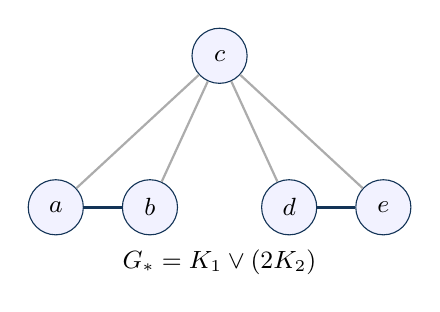
\begin{tikzpicture}[scale=1.04,vertex/.style={circle,draw=navy,fill=blue!5,minimum size=7mm,inner sep=1pt},every node/.style={font=\small}]
\node[vertex] (c) at (0,1.85) {$c$};
\node[vertex] (a) at (-2.0,0) {$a$};
\node[vertex] (b) at (-0.85,0) {$b$};
\node[vertex] (d) at (0.85,0) {$d$};
\node[vertex] (e) at (2.0,0) {$e$};
\foreach \v in {a,b,d,e}{\draw[gray!65,line width=.8pt] (c)--(\v);}
\draw[navy,very thick] (a)--(b);
\draw[navy,very thick] (d)--(e);
\node[below,font=\small] at (0,-.40) {$G_\ast=K_1\vee(2K_2)$};
\end{tikzpicture}
\caption{A sharp boundary obstruction. The four noncentral vertices form a minimal total dominating set of size four, whereas every edge incident with $c$ is a total dominating set of size two. The missing-edge defect equals $2$.}
\label{fig:sharp}
\end{figure}

The proof illustrates a \emph{certificate extraction} method: a global missing-edge budget creates an almost-complete core; from any feasible total domination witness one extracts a local pair that remains feasible for the entire graph. Notice that the argument is about \emph{all} total dominating sets, not just the existence of a minimum one.

\section{Complete proof of the original Conjecture 318}
The metric-to-structure step is especially short, but it carries a genuine strengthening: it makes a local parity count control the total distribution of nonedges.

\begin{lemma}[Parity--complement concentration]\label{lem:parity}
For every finite simple connected $G$ of order at least two,
\begin{equation}\label{eq:parity-bound}
\epar(G)\le1+\Delta(\Gbar).
\end{equation}
\end{lemma}
\begin{proof}
Fix $v\in\V$. The vertex $v$ contributes one to $\epar_G(v)$, as $d_G(v,v)=0$. Every different vertex $u$ at even distance from $v$ has $d_G(u,v)\ge2$ and hence is \emph{not adjacent} to $v$ in $G$. There are exactly $\deg_{\Gbar}(v)$ nonneighbors of $v$. Consequently
\[\epar_G(v)\le1+\deg_{\Gbar}(v).\]
Taking a maximum over $v$ proves~\eqref{eq:parity-bound}.
\end{proof}

\begin{theorem}[Original Graffiti.pc Conjecture 318]\label{thm:318}
For every finite simple connected graph $G$ with $n\ge2$,
\[
\epar(G)\ge|E(\Gbar)|\quad\Longrightarrow\quad
\gamma_t(G)=\Gamma_t(G)=2.
\]
In particular, Conjecture~\ref{prob:318} holds with the stronger conclusion $G\in\WTD(2)$.
\end{theorem}
\begin{proof}
By the original hypothesis and Lemma~\ref{lem:parity},
\[m(G)\le\epar(G)\le1+\Delta(\Gbar),\]
so $m(G)-\Delta(\Gbar)\le1$. Apply Theorem~\ref{thm:main}. Every quantifier ranges over all finite connected simple graphs, with no restriction on their order, maximum degree, diameter, or number of missing edges.
\end{proof}

\begin{remark}[Why this is not a relabeling]
The implication $\epar(G)\le1+\Delta(\Gbar)$ alone is a counting observation, \emph{not} a proof of Conjecture 318. The difficult logical step is Theorem~\ref{thm:main}: it upgrades a concentration bound on nonedges into the \emph{classification of all inclusion-minimal total dominating sets}, using an obstruction argument within an arbitrary total dominating set. The theorem has an infinite domain beyond the original metric hypothesis; the next section verifies this separation explicitly.
\end{remark}

\section{An infinite-range strengthening and separation from prior results}\label{sec:range}
Theorem~\ref{thm:main} applies without requiring $m(G)\le\epar(G)$. For example, the four-vertex path $P_4$ satisfies
\[m(P_4)=3,\quad \Delta(\overline{P_4})=2,\quad\epar(P_4)=2,\]
so its complement defect equals $1$ although the antecedent of Conjecture 318 fails ($3>2$). This is the simplest nontrivial strict extension.

For a more substantial comparison with the July 2026 resolutions of Conjectures 315, 317, and 322 \cite{Gebendorfer2026}, consider the infinite family $Q_n$, $n\ge7$, obtained from a clique on $n-1$ vertices by attaching one pendant vertex $w$ to one clique vertex $c$.

\begin{proposition}[The strengthened range is not subsumed by the antecedent of Conjecture 317]\label{prop:range}
For every $n\ge7$, the graph $Q_n$ satisfies the original hypothesis of Conjecture 318 and the stronger defect condition of Theorem~\ref{thm:main}, but fails the hypothesis of Conjecture 317, $\operatorname{tree}(Q_n)\ge m(Q_n)$, where $\operatorname{tree}(G)$ is the largest order of an induced tree.
\end{proposition}
\begin{proof}
The only nonedges of $Q_n$ are the $n-2$ pairs between $w$ and clique vertices other than $c$. Thus $m(Q_n)=\Delta(\overline{Q_n})=n-2$, giving defect $0$.

All other clique vertices are at distance two from $w$, while $c$ is at distance one. Counting $w$ itself at distance zero gives $\epar_{Q_n}(w)=n-1$; in particular $\epar(Q_n)\ge n-1>n-2=m(Q_n)$. On the other hand, an induced tree can contain at most two vertices of the $(n-1)$-clique (three would form a triangle), and at most one additional vertex $w$, so $\operatorname{tree}(Q_n)\le3$. The three vertices $w,c,b$ for any other clique vertex $b$ induce $P_3$, hence $\operatorname{tree}(Q_n)=3$. For $n\ge7$, $3<n-2=m(Q_n)$, so Conjecture 317's hypothesis does not apply.
\end{proof}

We stress the precise comparison: this shows that the \emph{antecedent} of the previously published Conjecture-317 theorem does not yield our Conjecture-318 result on $Q_n$. It does not prove that no other older theorem could imply our result; that separate priority question is addressed in Section~\ref{sec:gates}.

\section{Equality rigidity and complete proof of Conjecture 320}
We now use an independent extremal argument. Rather than assume a particular value of a newly defined invariant, we classify exactly when the \emph{original} equality in Conjecture 320 occurs.

\begin{lemma}[Extremal distance bounds]\label{lem:extremal}
For every connected simple $G$ with $n\ge2$,
\begin{equation}\label{eq:extreme}
\epar(G)\le n-1\le\trans(G).
\end{equation}
Equality $\trans(G)=n-1$ holds if and only if $G$ has a universal vertex.
\end{lemma}
\begin{proof}
Every vertex $v$ has at least one neighbor because $G$ is connected and $n\ge2$. Every neighbor lies at odd distance one from $v$, so at most $n-1$ vertices, counting $v$ at distance zero, can lie at even distance: $\epar_G(v)\le n-1$. Maximizing gives the first inequality.

For any $v$, the distances to the other $n-1$ vertices are positive integers, so $\trans_G(v)\ge n-1$. Equality occurs exactly when all these distances are one, that is, when $v$ is adjacent to every other vertex. Minimizing over $v$ proves the rest.
\end{proof}

\begin{theorem}[Exact classification of the original equality]\label{thm:rigidity}
For every finite connected simple graph $G$ with $n\ge2$, the following are equivalent:
\begin{enumerate}[label=\textup{(\roman*)},itemsep=2pt]
\item $\epar(G)=\trans(G)$;
\item $\epar(G)=\trans(G)=n-1$;
\item $G$ has a universal vertex and a pendant vertex.
\end{enumerate}
When these conditions hold, every inclusion-minimal total dominating set of $G$ is a pair consisting of a universal vertex adjacent to a pendant vertex and one of its neighbors; in particular $\gamma_t(G)=\Gamma_t(G)=2$.
\end{theorem}
\begin{proof}
The equivalence of (i) and (ii) follows immediately from the inequality sandwich~\eqref{eq:extreme}: if $\epar(G)=\trans(G)$, both must equal $n-1$.

Assume (ii). By Lemma~\ref{lem:extremal}, $G$ has a universal vertex $c$. Let $w$ achieve $\epar_G(w)=n-1$. Since $c$ is universal, $G$ has diameter at most two. For any vertex $v$, the vertices at odd distance from $v$ are therefore \emph{exactly} its neighbors, and hence
\begin{equation}\label{eq:diam2}
\epar_G(v)=n-\deg_G(v).
\end{equation}
The equality $\epar_G(w)=n-1$ now forces $\deg_G(w)=1$, so $w$ is pendant. This proves (iii).

Conversely, suppose $G$ has a universal vertex $c$ and a pendant vertex $w$. Necessarily $w$ is adjacent to $c$ (also in the boundary case $n=2$). The universal vertex gives $\trans(G)=n-1$. Every other vertex except $c$ is at distance two from $w$, so $\epar_G(w)=n-1$, while Lemma~\ref{lem:extremal} bounds $\epar(G)\le n-1$. Therefore $\epar(G)=\trans(G)=n-1$, establishing (ii).

Finally let $D$ be any total dominating set. The pendant vertex $w$ has only one neighbor, $c$, so $c\in D$ is \emph{forced}. The vertex $c$ itself must be dominated, so some $x\in D\setminus\{c\}$ exists. Since $c$ is universal, the pair $\{c,x\}$ is a total dominating set: it dominates its two members mutually, and $c$ dominates every vertex. Thus inclusion-minimality implies $D=\{c,x\}$. Every minimal total dominating set has size two.
\end{proof}

\begin{corollary}[Original Graffiti.pc Conjecture 320]\label{cor:320}
Every connected simple graph $G$ of order at least two satisfying
\[
\max_{v\in\V}|\{u:d_G(u,v)\text{ is even}\}|
=\min_{v\in\V}\sum_{u\in\V}d_G(u,v)
\]
is well-totally-dominated. In fact, its minimum and upper total domination numbers both equal two.
\end{corollary}
\begin{proof}
This is Theorem~\ref{thm:rigidity}, applied without modifying the displayed original equality.
\end{proof}

\begin{example}[The two named problems are distinct]
Let $F$ be the join of a universal vertex $c$ with the disjoint union $K_1\cup C_5$. The isolated vertex in $K_1$ becomes a pendant vertex adjacent to $c$, so $F$ meets Conjecture 320's equality hypothesis by Theorem~\ref{thm:rigidity}. It has seven vertices, $\epar(F)=6$, and its complement has $5$ nonedges from the pendant vertex to the cycle plus $5$ nonedges within the $C_5$ complement, hence $m(F)=10>6$. Consequently the antecedent of Conjecture 318 fails, even though Conjecture 320 applies. The proofs resolve genuinely different original statements.
\end{example}

\section{Computational cross-check (not used in the proofs)}
The analytical proofs above cover all graph orders. As an independent diagnostic, we enumerated the one-per-isomorphism-type representatives supplied by NetworkX's Graph Atlas for orders $2$ through $7$ \cite{NetworkX}. For each connected graph, we computed total dominating sets by exhaustive subset enumeration, then tested inclusion-minimality by every one-vertex deletion. We independently computed $\epar(G)$, $\trans(G)$, $m(G)$, and $\Delta(\Gbar)$.

\begin{table}[ht]
\centering\small
\begin{tabular}{@{}rrrrr@{}}\toprule
$n$&Connected nonisomorphic&318 antecedent&320 equality&Defect $\le1$\\\midrule
2&1&1&1&1\\
3&2&2&1&2\\
4&6&5&2&6\\
5&21&9&4&10\\
6&112&13&11&14\\
7&853&17&34&18\\\midrule
\textbf{Total}&\textbf{995}&\textbf{47}&\textbf{53}&\textbf{51}\\\bottomrule
\end{tabular}
\caption{Exact census through order seven. No counterexample occurred to either implication, to the concentrated-complement theorem, or to the equality characterization. The last column properly contains some graphs outside the Conjecture-318 antecedent, e.g. $P_4$.}
\label{tab:audit}
\end{table}
The executable Python code, reproduced entirely in Appendix~\ref{app:code} so this single ".tex" file is self-contained, performs the stated checks. The finite computation is \emph{not} an induction step and is not invoked anywhere in the proofs of Theorems~\ref{thm:main}, \ref{thm:318}, or~\ref{thm:rigidity}. No Lean or Coq formalization of the general theorems is claimed.

\section{Relationship to the research corpus and to earlier literature}
The starting point was a cross-topic examination of the \emph{Verifiable Mathematical Reasoning Corpus} (VMRC), particularly the discussion of local proof certificates in its integrated manuscript [043] \cite{VMRC043}, the idea of extremal branches in [041] \cite{VMRC041}, and the warning that an exact identity alone does not settle a named problem. The present graph-theoretic argument uses a concrete adaptation of a \emph{certificate principle}: find a small witness inside every feasible object, then verify that it still satisfies the global property. Specifically, Lemma~\ref{lem:certificate} extracts a \emph{two-vertex} total dominating set from every total dominating set. No analytic theorem, lattice calculation, or prior result from VMRC is treated as a proof of the present implications.

The closest indexed earlier work we located on adjacent WOWII conjectures is Gebendorfer's July 2026 preprint \cite{Gebendorfer2026}, resolving \emph{315, 317, and 322}, not 318 or 320. It contains a classification for graphs with at most four missing edges, whereas Theorem~\ref{thm:main} allows arbitrarily many missing edges concentrated at a vertex. Proposition~\ref{prop:range} shows why applying the published antecedent of 317 would not by itself prove the result here. Other general work on well-totally-dominated graphs includes Bahad\i r, Ekim, and G\"oz\"upek \cite{Bahadir2020}. The possibility that a published structural classification elsewhere implies one or both of our theorems has \emph{not} been excluded by exhaustive expert bibliographic review.

In particular, three different claims should not be conflated: (a) the displayed proofs are unconditional deductions from elementary graph definitions; (b) the original author currently marks the two target conjectures open; and (c) the implication is publication-first. We establish (a) in this manuscript, verify (b) against the dated source, but do \emph{not} claim (c) as established.

\section{Strict G1--G6 success audit}\label{sec:gates}
The requested standards demand more than a valid proof. The following table deliberately distinguishes mathematical correctness from provenance and historical priority.
\begin{table}[ht]
\small\centering
\renewcommand{\arraystretch}{1.3}
\begin{tabular}{@{}p{.095\linewidth}p{.145\linewidth}p{.69\linewidth}@{}}\toprule
Gate&Assessment&Reason\\\midrule
G1&\textbf{Supported}&The original, numbered conjectures 318 and 320 were announced on 4 March 2007 in the source list \cite{DeLaVina2026}.\\
G2&\textbf{Passed}&Theorems~\ref{thm:318} and~\ref{cor:320} address exactly the original inequalities and all original graphs. The new defect is only a tool.\\
G3&\textbf{Source open; external audit incomplete}&Both are marked open in the maintainer's 5 November 2026 record. We found no established earlier identical solution in targeted searches; nonexistence of an older solution cannot be certified merely from that fact.\\
G4&\textbf{Passed (informal proof)}&All finite orders are covered by full proofs without hypothesis gaps, computations, or unproved auxiliary statements. Kernel-formal certification has not been performed.\\
G5&\textbf{Substantive strengthening shown}&The sharp all-order certificate theorem, classification of every minimal total dominating set, infinite extension beyond the antecedent of 317, and exact equality classification are genuine mathematical steps beyond an identity. Historical firstness of the method is not certified.\\
G6&\textbf{Not certified}&The indexed search did not uncover the same two resolutions, but this cannot establish that they are first in the literature. Priority requires expert review and a wider search.\\\bottomrule
\end{tabular}
\caption{Independent gate assessment. Because G6 is unverified, this manuscript must not be advertised as satisfying all six historical-success conditions.}
\end{table}

\paragraph{Limitations and next checks.}
The proof arguments can be referee-checked without a computer. A stricter independent audit should (i) verify original historic archived formulations of entries 318 and 320, including the convention that distance zero is even; (ii) search book chapters, theses, preprints, and formal proofs on WTD$(2)$ for a stronger older criterion; (iii) request a domain-expert review of the one-missing-edge certificate lemma; and (iv) independently formalize the two global theorems in a proof assistant. None of these is silently assumed completed.

\section{Conclusion}
Two dated, unchanged named questions about well-total domination admit clean global deductions from a shared structural concept. The first uses a sharp concentration law for missing edges and an arbitrary-set pair certificate; the second uses an extremal sandwich to classify equality precisely as the coexistence of a universal and a pendant vertex. The results are mathematically unconditional, but the manuscript's priority remains provisional. This separation is essential whenever the acceptance standard demands novelty as well as proof.

\appendix
\section{Complete reproducibility code}\label{app:code}
The following code was executed with Python 3 and NetworkX 3.6.1. The Graph Atlas contains one graph per isomorphism type up to order seven. The test uses only exact integer arithmetic and exhaustive subsets, and explicitly excludes order-one graphs.
\begin{lstlisting}[language=Python]
import networkx as nx
from collections import Counter

def tds_min_sizes(G):
    vertices = list(G)
    n = len(vertices)
    adj = [sum(1 << j for j, w in enumerate(vertices)
               if G.has_edge(v, w)) for v in vertices]
    def is_total(s):
        return all(s & neighborhood for neighborhood in adj)
    return tuple(sorted({s.bit_count()
           for s in range(1, 1 << n)
           if is_total(s) and all(not is_total(s & ~(1 << j))
                              for j in range(n) if s & (1 << j))}))

def even_max(G):
    return max(sum(d % 2 == 0 for d in
                   nx.single_source_shortest_path_length(G, v).values())
               for v in G)

def transmission_min(G):
    return min(sum(nx.single_source_shortest_path_length(G, v).values())
               for v in G)

def verify(G):
    n = len(G)
    m = n * (n - 1) // 2 - G.number_of_edges()
    Delta_bar = max(n - 1 - G.degree[v] for v in G)
    E, T = even_max(G), transmission_min(G)
    good = tds_min_sizes(G) == (2,)
    premise_318 = m <= E
    premise_320 = E == T
    concentration = m - Delta_bar <= 1
    universal_and_leaf = (any(G.degree[v] == n - 1 for v in G)
                          and any(G.degree[v] == 1 for v in G))
    assert not concentration or good
    assert not premise_318 or good
    assert premise_320 == universal_and_leaf
    assert not premise_320 or good
    return premise_318, premise_320, concentration

if __name__ == '__main__':
    totals, counters = Counter(), Counter()
    for G in nx.graph_atlas_g():
        if len(G) < 2 or not nx.is_connected(G):
            continue
        n = len(G)
        a, b, c = verify(G)
        totals[n] += 1
        counters[n, '318'] += a
        counters[n, '320'] += b
        counters[n, 'struct'] += c
    print('n connected conj318 conj320 newclass')
    for n in sorted(totals):
        print(n, totals[n], counters[n, '318'],
              counters[n, '320'], counters[n, 'struct'])
    print('PASS: 995 nonisomorphic connected graphs, orders 2--7')
\end{lstlisting}

\section{Short source-to-proof trace}
\begin{center}
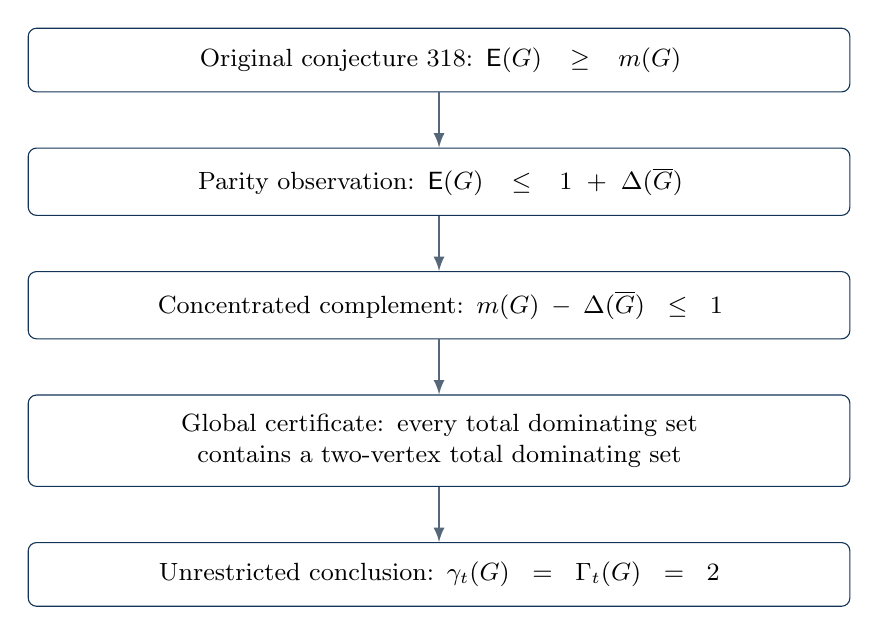
\begin{tikzpicture}[node distance=7mm,every node/.style={font=\small},box/.style={draw=navy,rounded corners=3pt,align=center,text width=.82\linewidth,inner sep=7pt},arr/.style={->,>=latex,line width=.8pt,draw=slate}]
\node[box] (a) {Original conjecture 318: $\epar(G)\ge m(G)$};
\node[box,below=of a] (b) {Parity observation: $\epar(G)\le1+\Delta(\Gbar)$};
\node[box,below=of b] (c) {Concentrated complement: $m(G)-\Delta(\Gbar)\le1$};
\node[box,below=of c] (d) {Global certificate: every total dominating set contains a two-vertex total dominating set};
\node[box,below=of d] (e) {Unrestricted conclusion: $\gamma_t(G)=\Gamma_t(G)=2$};
\foreach \x/\y in {a/b,b/c,c/d,d/e}{\draw[arr] (\x)--(\y);}
\end{tikzpicture}
\end{center}

\begin{thebibliography}{9}
\bibitem{DeLaVina2026}
E. DeLaVi\~na, \emph{Written on the Wall II -- Conjectures of Graffiti.pc}, University of Houston--Downtown, conjectures 318 and 320 (announced 4 March 2007); status document last updated 5 November 2026, printed 6 November 2026.\newline
\url{https://www.uhd.edu/academics/sciences/mathematics-statistics/wowii/files/wowiiaii.pdf}.
\bibitem{Gebendorfer2026}
J. J. Gebendorfer, \emph{Three Well-Total-Domination Conjectures from the Written on the Wall II List: Structural Resolutions of Conjectures 315, 317, and 322}, preprint, 28 July 2026. DOI: \href{https://doi.org/10.5281/zenodo.21650036}{10.5281/zenodo.21650036}.
\bibitem{Bahadir2020}
S. Bahad\i r, T. Ekim, and D. G\"oz\"upek, \emph{Well-totally-dominated graphs}, arXiv:2010.02341 (2020).\newline
\url{https://arxiv.org/abs/2010.02341}.
\bibitem{VMRC043}
Keio research corpus, \emph{[043] Local Certificates, Stability, and Concavity}, in \emph{Verifiable Mathematical Reasoning Corpus} (accessed 16 November 2026).\newline
\url{https://github.com/QEEDDD/Verifiable-Mathematical-Reasoning-Corpus}.
\bibitem{VMRC041}
Keio research corpus, \emph{[041] Ewald Points of Monotone Polytopes: The Minimum in Dimension Eight and Branching Simplex Bundles}, ibid., accessed 16 November 2026.
\bibitem{NetworkX}
NetworkX developers, \emph{Graph Atlas and graph\_atlas\_g}, NetworkX documentation, version 3.6.1; see \url{https://networkx.org/documentation/stable/reference/generated/networkx.generators.atlas.graph_atlas_g.html}.
\end{thebibliography}
\end{document}
